\chapter{Ergebniss}

Die in der Stuide getesteten Probanden waren Studenten der TU München und wiesen die folgende Werte auf:

    \begin{itemize}
        \item 35,9 Prozent von ihnen waren weiblich 
        \item die Probanden kamen überwiegend aus Bayern 66,7 Prozent
        \item das Druchschnittsalter lag bei 21,2 Jahren 
        \item die Studenten waren im Mittel im 3,85. Fachsemester
    \end{itemize}

 Um die Forschungsfrage (1) zu untersuchen, wurden Gruppen mit Hilfe einer Varianzanalyse auf folgende Werte untersucht: Fixationen auf dem Bild, Fixationen auf dem Text, Dauer des ersten Durchgangs, sowie der Dauer des zweiten Durchgangs untersucht.


\begin{figure}[!ht]
\noindent\hspace{0.5mm}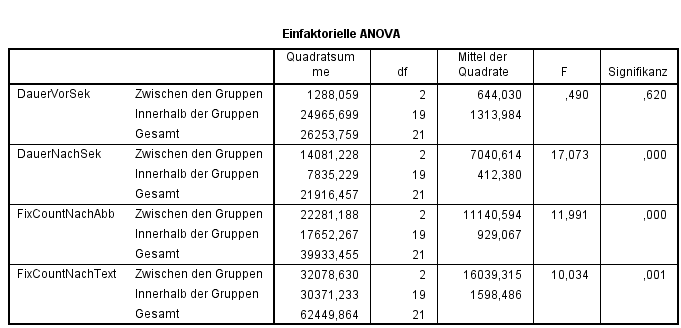
\includegraphics[width=15cm]{./Ressourcen/Gruppenunterscheidung.png}
\caption{Gruppenvarianz, Lorenz Müller}
\end{figure}

Wenn man sich der zweiten Forschungsfrage widment, kommt man zu folgenden Ergebnissen:
Alle Studenten erzielten im Schnitt 6,03 Punkte. 
Die jeweiligen Gruppen erzielten für die Bearbeitung alle Aufgaben im Durchschnitt folgende Punkte:

\begin{table}[!h]
\hspace{-5pt}
\begin{tabularx}{\textwidth + 5pt}{| @{\hspace{3pt}} M || @{\hspace{3pt}} M  | @{\hspace{3pt}} M | @{\hspace{3pt}} M |}
\hline
\textbf{ } & \textbf{Typ Unsicher} & \textbf{Typ Problemlöser} & \textbf{Typ Textuell}\\
\hline
\hline
Punkte        & 6,17 & 5,5 & 6,3\\
\hline
\end{tabularx}
\caption{Mittelwert der Punkte}
\end{table}


Bei der Untesuchung nach signifikanten Unterschieden, wurde
die Varianzanalyse über die Gesamtpunktzahl gestellt, welche folgende Ergebnisse hervorbringt:

\begin{figure}[!ht]
\noindent\hspace{0.5mm}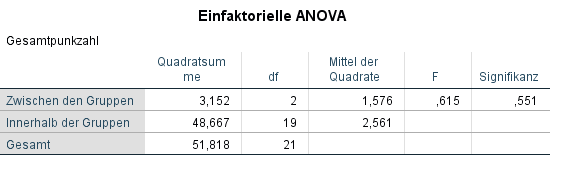
\includegraphics[width=15cm]{./Ressourcen/Punktevarianz.png}
\caption{Punktevarianz, Lorenz Müller}
\end{figure}

Widmet man sich nun der dritten Forschungsfrage, desm Einflusses der gewählten Bilder zu, ergibt sich.
Betrachtet man die Beantwortung der einzelnen Aufgaben von allen Probanden.

\begin{table}[!h]
\hspace{-5pt}
\begin{tabularx}{\textwidth + 5pt}{| @{\hspace{3pt}} M || @{\hspace{3pt}} M  | @{\hspace{3pt}} M | @{\hspace{3pt}} M |}
\hline
\textbf{Aufgabe} & \textbf{Radfahrerin 1} & \textbf{Radfahrerin 2} & \textbf{Rennfahrer} \\
\hline
\hline
Prozent richtig beantwortet       & 97,5 & 17,9 & 76,9 \\
\hline
\end{tabularx}
\caption{Mittelwert der Punkte}
\end{table}

\begin{table}[!h]
\hspace{-5pt}
\begin{tabularx}{\textwidth + 5pt}{| @{\hspace{3pt}} M | @{\hspace{3pt}} M  | @{\hspace{3pt}} M | @{\hspace{3pt}} M |}
\hline
\textbf{Zufall} & \textbf{Berg 1} & \textbf{Berg 2} & \textbf{Autofahren}\\
\hline
\hline
    51,3 & 76,9 & 74,3 &  94,9\\
\hline
\end{tabularx}
\caption{Mittelwert der Punkte}
\end{table}

Im Schnitt wurden somit die jeweiligen Bildtypen zu folgenden Prozentwerten richtig beantwortet. 

\begin{table}[!h]
\hspace{-5pt}
\begin{tabularx}{\textwidth + 5pt}{| @{\hspace{3pt}} M || @{\hspace{3pt}} M  | @{\hspace{3pt}} M | @{\hspace{3pt}} M |}
\hline
\textbf{Aufgabentyp} & \textbf{dekorativ} & \textbf{essenziell} \\
\hline
\hline
Prozent richtig beantwortet       & 66,7 & 74,3 \\
\hline
\end{tabularx}
\caption{Mittelwert der Punkte}
\end{table}

Bei der Untersuchung nach signifikanten Unterschieden ergibt sich bei der Varianzanalyse:


\begin{figure}[!ht]
\noindent\hspace{0.5mm}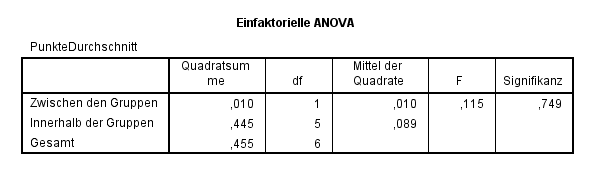
\includegraphics[width=15cm]{./Ressourcen/Aufgabenuntescheidung.png}
\caption{Punktevarianz, Lorenz Müller}
\end{figure}




Widmet man sich nun der vierten Forschungsfrage:
Werden bei der Auswetung der einzelnen Gruppen auf die Fragen Ergebnisse fett markiert, welche sich um mehr als 20 Prozent vom Wert der Allgemeinheit unterscheiden:

\begin{table}[!h]
\hspace{-5pt}
\begin{tabularx}{\textwidth + 5pt}{| @{\hspace{3pt}} M || @{\hspace{3pt}} M  | @{\hspace{3pt}} M | @{\hspace{3pt}} M |}
\hline
\textbf{Aufgabe} & \textbf{Radfahrerin 1} & \textbf{Radfahrerin 2} & \textbf{Rennfahrer} \\
\hline
\hline
Prozent richtig beantwortet       & 100 & 10 & 90 \\
\hline
\end{tabularx}
\caption{Typ Problemlöser bei den unteschiedlichen Aufgabenstellungen 1}
\end{table}


\begin{table}[!h]
\hspace{-5pt}
\begin{tabularx}{\textwidth + 5pt}{| @{\hspace{3pt}} M | @{\hspace{3pt}} M  | @{\hspace{3pt}} M | @{\hspace{3pt}} M |}
\hline
\textbf{Zufall} & \textbf{Berg 1} & \textbf{Berg 2} & \textbf{Autofahren}\\
\hline
\hline
    40 & 60 & 70 &  \textbf{50}\\
\hline
\end{tabularx}
\caption{Typ Problemlöser bei den unteschiedlichen Aufgabenstellungen 2}
\end{table}

\begin{table}[!h]
\hspace{-5pt}
\begin{tabularx}{\textwidth + 5pt}{| @{\hspace{3pt}} M || @{\hspace{3pt}} M  | @{\hspace{3pt}} M | @{\hspace{3pt}} M |}
\hline
\textbf{Aufgabe} & \textbf{Radfahrerin 1} & \textbf{Radfahrerin 2} & \textbf{Rennfahrer} \\
\hline
\hline
Prozent richtig beantwortet       & 83 & 17 & 67 \\
\hline
\end{tabularx}
\caption{Typ Unsicher bei den unteschiedlichen Aufgabenstellungen 1}
\end{table}

\begin{table}[!h]
\hspace{-5pt}
\begin{tabularx}{\textwidth + 5pt}{| @{\hspace{3pt}} M | @{\hspace{3pt}} M  | @{\hspace{3pt}} M | @{\hspace{3pt}} M |}
\hline
\textbf{Zufall} & \textbf{Berg 1} & \textbf{Berg 2} & \textbf{Autofahren}\\
\hline
\hline
    \textbf{83} & 83 & 67 &  100\\
\hline
\end{tabularx}
\caption{Typ Unsicher bei den unteschiedlichen Aufgabenstellungen 2}
\end{table}

\begin{table}[!h]
\hspace{-5pt}
\begin{tabularx}{\textwidth + 5pt}{| @{\hspace{3pt}} M || @{\hspace{3pt}} M  | @{\hspace{3pt}} M | @{\hspace{3pt}} M |}
\hline
\textbf{Aufgabe} & \textbf{Radfahrerin 1} & \textbf{Radfahrerin 2} & \textbf{Rennfahrer} \\
\hline
\hline
Prozent richtig beantwortet       & 100 & 17 & \textbf{100} \\
\hline
\end{tabularx}
\caption{Typ Textuell bei den unteschiedlichen Aufgabenstellungen 1}
\end{table}


\begin{table}[!h]
\hspace{-5pt}
\begin{tabularx}{\textwidth + 5pt}{| @{\hspace{3pt}} M | @{\hspace{3pt}} M  | @{\hspace{3pt}} M | @{\hspace{3pt}} M |}
\hline
\textbf{Zufall} & \textbf{Berg 1} & \textbf{Berg 2} & \textbf{Autofahren}\\
\hline
\hline
    67 & 67 & 67 &  83\\
\hline
\end{tabularx}
\caption{Typ Textuell bei den unteschiedlichen Aufgabenstellungen 2}
\end{table}

Somit sind diejenigen Ergebnisse auffälig, wobei mit Hilfe der Varianzanalyse untersucht wurde, ob sich diese signifikant unterscheiden: 

\begin{itemize}
    \item Autofahrt wurde von dem Typ Problemlöser mit nur 50 Prozent richtig gelöst. (Allgemeinheit 94,9 Prozent) ($\alpha$ = 0,243 F = 1,407)
    \item Zufall wurde von dem Typ Unsicher mit 83,3 Prozent richtig gelöst. (Allgemeinheit 0,513) ($\alpha$ = 0,152 F = 2,135)
    \item Rennfahrer wurde von Typ Textuell von allen Probanden richtig gelöst. (Allgemeinheit 0,769) ($\alpha$ = 0,092 F = 2,990)
\end{itemize}

Betrachtet man noch abschliesend, wie sich die unterschiedlichen Lerntypen mit den Bildtypen verhalten haben, so ergibt sich folgende Tabelle.

\begin{table}[!h]
\hspace{-5pt}
\begin{tabularx}{\textwidth + 5pt}{| @{\hspace{3pt}} M | @{\hspace{3pt}} M  | @{\hspace{3pt}} M | @{\hspace{3pt}} M |}
\hline
\textbf{Lerntyp} & \textbf{Unsicher} & \textbf{Problemlöser} & \textbf{Textuell}\\
\hline
\hline
    dekorativ & 62,5 & 60 &  62,5\\
\hline
    essenziell & 83,3 & 60,0 &  83,3\\
\hline
\end{tabularx}
\caption{Typ Textuell bei den unteschiedlichen Aufgabenstellungen 2}
\end{table}

Mit der Varianzanalyse: 

\begin{figure}[!ht]
\noindent\hspace{0.5mm}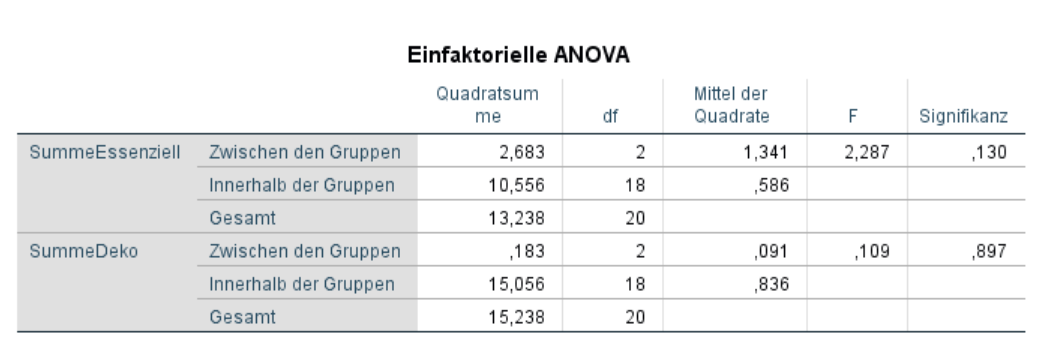
\includegraphics[width=15cm]{./Ressourcen/DekoEssGruppen.png}
\caption{Punktevarianz, Lorenz Müller}
\end{figure}


